\section{6DOF Dynamics and Transfer Functions}
\label{sec:dyn}

The 6DOF model (\texttt{Dinamica6DOF.slx} and, in closed loop, \texttt{GuiamentoControle.slx}) integrates the six rigid-body equations with variable mass and inertia, summing aerodynamic, propulsive and gravitational forces and moments in the body frame.

\subsection{Short-Period Linearization}

\texttt{FTransDin.m} linearizes the pitch (short-period) motion about $\alpha=0$, producing four second-order transfer functions with input equal to the fin deflection $\delta$:

\begin{table}[H]
\centering
\caption{Short-period transfer functions.}
\begin{tabular}{lll}
\toprule
Transfer function & Output & Use \\
\midrule
$\delta\rightarrow q$ & pitch rate & inner rate-gyro loop \\
$\delta\rightarrow\theta$ & attitude ($=q\cdot 1/s$) & outer attitude loop \\
$\delta\rightarrow\alpha$ & angle of attack & --- \\
$\delta\rightarrow A_z$ & lateral acceleration & acceleration loop \\
\bottomrule
\end{tabular}
\end{table}

The moment transfer from the DATCOM reference to the real CG is
\[
    \Delta x_{CG}=\frac{x_{CG}-x_{CRM}}{D_{ref}}
    \quad\Rightarrow\quad
    C_{m\alpha}=\frac{dC_M}{d\alpha}+\Delta x_{CG}\,C_{z\alpha}.
\]

\subsection{Why the Airframe Needs an Autopilot}

The bare airframe is lightly damped: $\xi\approx 0.08$ in open loop, so a fin deflection excites an oscillation that takes long to decay, and $\omega_n\propto\sqrt{\bar q}$ rises with speed. The acceleration channel additionally has a non-minimum-phase zero at $\approx+13.7~\text{rad/s}$, which produces the initial dip in the acceleration step and limits the achievable bandwidth. The inner rate-gyro loop feeds back $q$ and raises the damping from $\xi\approx 0.08$ to $\approx 1$.

\begin{figure}[H]
\centering
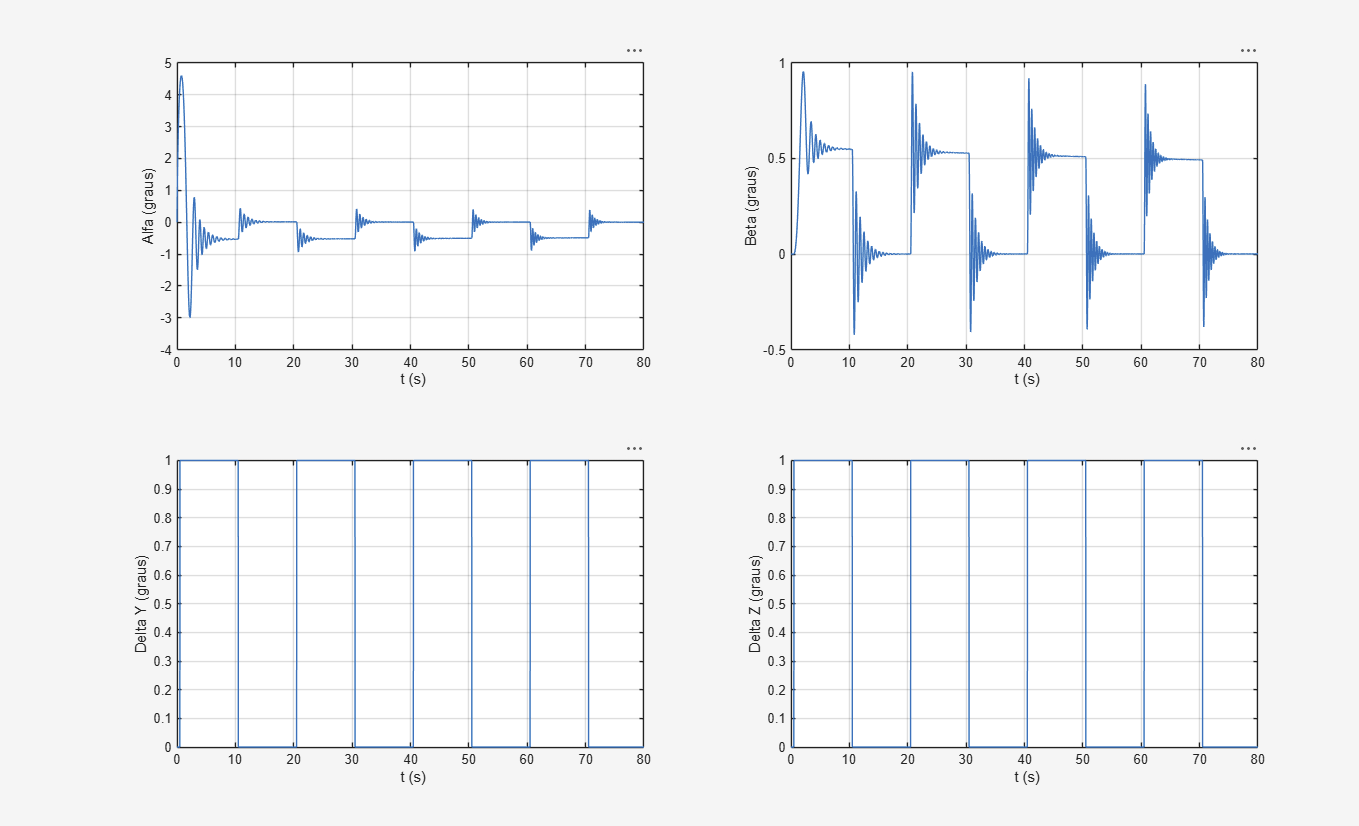
\includegraphics[width=0.82\textwidth]{figures/airframe_free_response.png}
\caption{Open-loop free response of the airframe to a train of fin steps: $\alpha$ and $\beta$ oscillate and decay slowly (short-period damping $\xi\approx 0.08$), with the frequency rising as the missile accelerates. This lightly damped behavior is what the autopilot must correct.}
\end{figure}
